\documentclass[a4paper,english,12pt,bibliography=totoc]{scrreprt}

\usepackage[T1]{fontenc} %immer
\usepackage[utf8]{inputenc} %am
\usepackage{babel} %Anfang

\usepackage{enumitem} %Aufzählungen verändern

%Gleichungen verwenden
\usepackage{newtxtext}
\usepackage{amsmath}
\usepackage{amssymb}
\usepackage{mathptmx}
%\usepackage{txfonts}

\usepackage{listings}% code blocks
\usepackage[most]{tcolorbox}

%Querverweise
\usepackage{varioref} %immer
\usepackage{hyperref} %in dieser
\usepackage{cleveref} %Reihenfolge

\usepackage{booktabs} %schönere Tabellen
\usepackage{siunitx} %SI-Einheiten
\usepackage{tabularx} %Tabellen mit flexiblen Spalten	

\usepackage{graphicx} %Grafiken verwenden

\usepackage[backend=biber,style=numeric]{biblatex}
\addbibresource{References.bib} 

\usepackage{lipsum} %Blindtext
\usepackage{subcaption}
\usepackage{afterpage}
\usepackage[headsepline]{scrlayer-scrpage} %Paket für Kopfzeilen
\usepackage{afterpage}
\usepackage{float}
\automark[subsection]{section}

\pagestyle{scrheadings}
\ihead{} % oben links
\chead{\leftmark} % oben Mitte
\ohead{} % oben rechts
\cfoot{\pagemark} % unten Mitte
\automark[section]{section} % Modified line

% Zu volle hboxen korrigieren
\tolerance 1414
\hbadness 1414
\emergencystretch 1.5em
\hfuzz 0.3pt
\widowpenalty=10000
\vfuzz \hfuzz
\raggedbottom

%Informationen über das Dokument
\date{\today}


\begin{document}


\begin{titlepage}
	\centering
	
\includegraphics[width=0.8\textwidth]{logo_uulm_sw}
	
	\vspace{1cm}
	\LARGE Laboratory Module for Master Programs
	\Huge \textbf{Biophysics Lab Course}
	
	\vspace{1cm}
	\Large Experiment:

	\Huge \textbf{Gene Expression}
	
	\vspace{15mm}
	\Large Performed on 
	
	\vspace{5mm}
	\LARGE Group 8
	
	\vspace{1cm}
	\Large
	\begin{tabular}{rcl}
	\textbf{Haiyang Zhang} & and & \textbf{Nicolae Turcan}\\
	\href{mailto:student.1@uni-ulm.de}{haiyang.zhang@uni-ulm.de} & & \href{mailto:student.2@uni-ulm.de}{nicolae.turcan@uni-ulm.de}
	\end{tabular}
	
	\vspace{7mm}
	Supervisor: Camilla Förster
	
	\vfill
	\begin{tabular}{p{50mm}@{\hspace{5cm}}p{50mm}}
	\hrulefill & \hrulefill \\
	%\centering Haiyang Zhang  & \centering Nicolae Turcan
	\end{tabular}
	
	\vspace{5mm}
	\normalsize \raggedright
	We hereby confirm that we have elaborated the present work independently and have detailed knowledge of the entire contents.
\end{titlepage}



\tableofcontents

%COMMENTS BY CAMILLA
%- Aim: What was the aim of the experiment, how was it to be achieved?
%- !NO introduction, NO theory section, NO methods section
%- Results section with a brief description of what was done to achieve the results shown and of course show and describe your results
%- Detailed captions, from which it is also clear what is shown
%- Discussion and classification of the results

%Formalities: Cover sheet with group number and name, declaration of independence, page number


\chapter{Abstract}
\label{cha:Abstract & Aim}

% a short paragraph on the aim of the lab, then what current knowledge was used to achieve this task and finally how this result is important and it´s applications. 

This laboratory experiment aimed to investigate the expression and photoconversion properties of the Eos fluorescent protein in \textit{E. coli}. Utilizing fundamental techniques in molecular biology and fluorescence spectroscopy, we transformed competent \textit{E. coli} cells with the pQE32-Eos plasmid, induced protein expression, and purified the resultant protein. The photoconversion from green to red fluorescence upon UV light exposure was then analyzed. Understanding the photoconversion properties of EosFP has significant implications for its application in advanced fluorescence microscopy and molecular tracking in cell biology.

  

\chapter{Experiment}
\label{cha:Experiment}

%Briefly descirbe the experiment steps and the reasons to do so. The amount and time could be attached to the compounds and operations with ().
The experiment was conducted over four days. The task of the first day was to transform the plasmid to \textit{E.coli}. Two groups of \textit{E.coli} (sample and negative control) were prepared. 1 \textmu l of plasmid was put into the sample group to observe the influence of plasmid by comparing the bacteria in two groups. Then a heat shock (5 min ice incubation -- 42 \textdegree C for 45 sec -- 5 min ice incubation) was applied to both group to help the transformation of the plasmid. After that, sterile LB (1ml) was added, providing nutrition for bacteria growth. Finally, the two groups of bacteria were spread on two agar plates separately and incubated overnight at 37 \textdegree C. The agar plates were filled with LB (25 ml), ampicillin (50 \textmu l) and kanamycin (25 \textmu l). Ampicillin and kanamycin are two types of antibiotics. The \textit{E.coli} M15 has antibiotic resistance towards kanamycin but not towards ampicillin, while the plasmid pQE32 transformed \textit{E.coli} could also survive with ampicillin. In this way, if we see colonies only in the sample group, we could say that the plasmid was transformed successfully.\\

\begin{figure}[H]
    \centering
    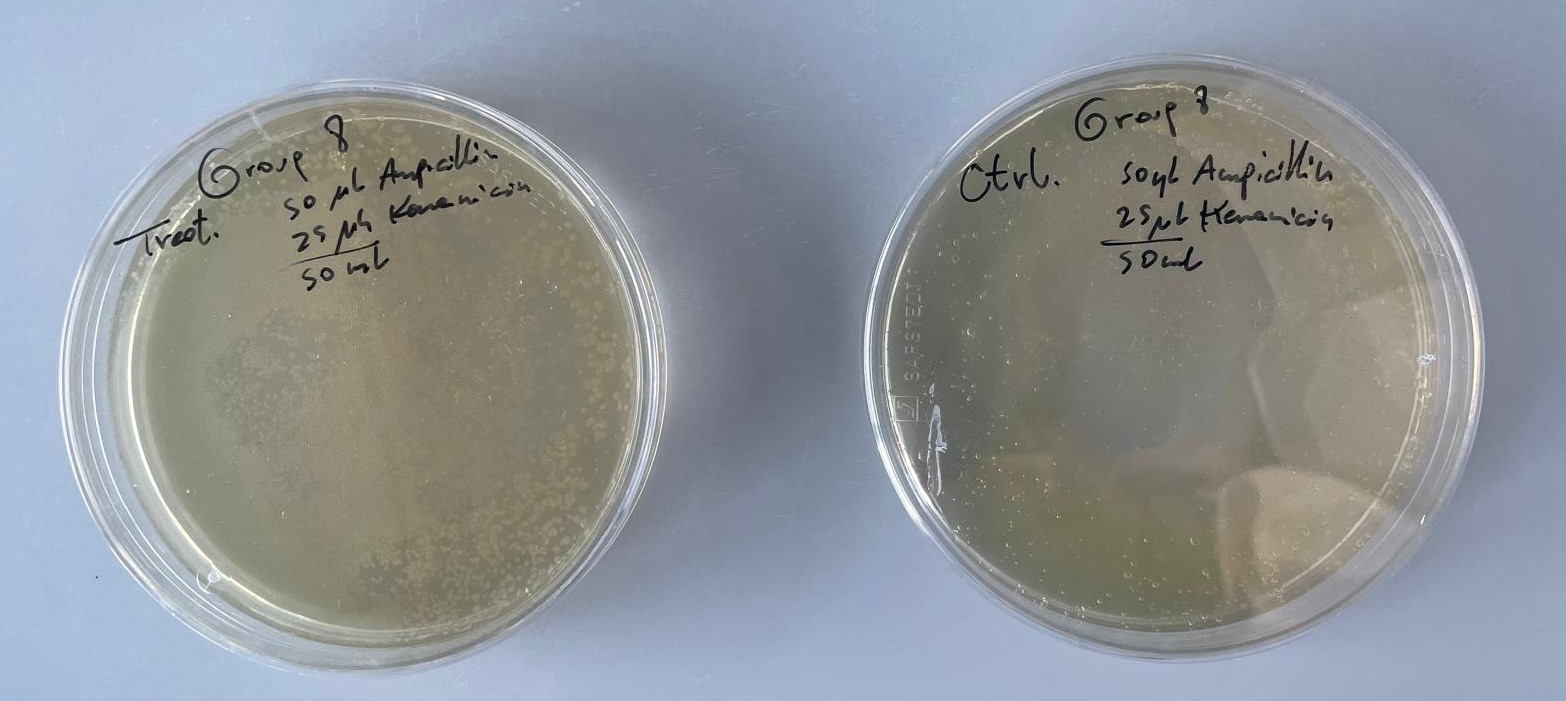
\includegraphics[width = 0.8\textwidth]{Figures/agarplates.jpeg}
    \caption{The treatment and control agar plates,
    the Treatment Group shows many  white dots that correspond to bacterial colonies where as the control plate, which  regretfully contains bubbles and has a less even surface, doesn't display any colonies}
    \label{fig:enter-label}
\end{figure}



On the second day, we aimed to inoculate the bacteria and induce the target gene expression. In the morning, we inoculated the bacteria from the sample group to the new environment (5 ml sterile LB, 5 \textmu l ampicillin, and 2.5 \textmu l kanamycin). We put them in the incubator, to promote the bacteria growth(37 \textdegree C, 200 rpm, 6 h). In the afternoon, the bacteria solution was inoculated again (100 ml sterile LB, 100 \textmu l ampicillin, and 50 \textmu l kanamycin) and cultivated (37 \textdegree C, 200 rpm). During this period, we measured the optical density of bacteria solution at 600 nm ($\mathrm{OD_{600}}$) every 20 minutes, until its $\mathrm{OD_{600}}$ reached 0.5 but less than 0.7. Optical density 600 nm is the negative logarithm of the transmission coefficient at 600 nm. It is used as a signal of bacteria concentration in the solution. By plotting the relationship of $\mathrm{OD_{600}}$ over time (Figure 2.1), we could infer the reproduction situation of bacteria. In this experiment, when it was located between 0.5 and 0.7, we thought that we reached the target bacteria concentration. After that, 100  \textmu l IPTG (Isopropyl $\beta$ -D-1-thiogalactopyranoside) inducing the gene expression in \textit{E.coli} was applied to promote the transcription by influencing the lac operon. Finally, the bacteria solution was put in the incubator (25 \textdegree C, >12 h) again to generate more protein in the system.\\

\begin{figure}[H]
    \centering
    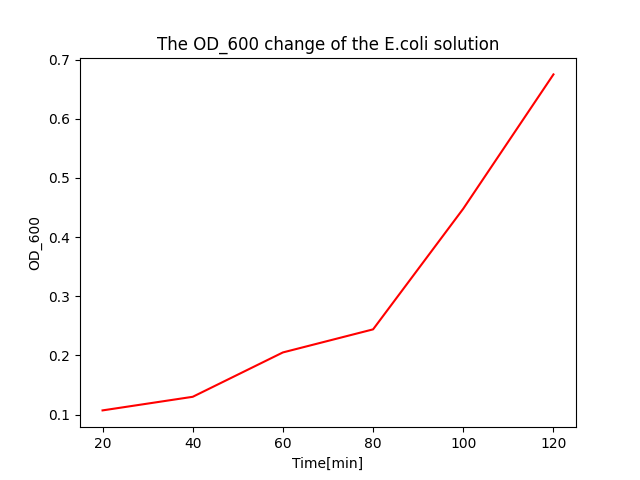
\includegraphics[width = 0.8\textwidth]{Figures/OD_600.png}
    \caption{The Optical Density at 600 nm over time}
    \label{fig:enter-label}
\end{figure}

On the third day, we purified the protein by chromatography and quantified it by its absorption spectrum and Beer-Lambert law. In the morning, we harvested the protein by centrifuging the bacteria, lysing the bacteria by sonicator (4x15 sec 30\%power, 30 sec pause between each group), and centrifuging the cell lysis (20 min, 20.000x g, 4 \textdegree C). Afterward, we applied nickel affinity chromatography to precisely acquire the target protein(Eos FP). Eos contains a so-called His-tag, which binds specifically to nickel on one of its terminal ends. However, the Eos FP could also be eluted from the nickel binding by imidazole, which could displace the His-tagged protein from the nickel. In our experiment, we applied some resin beads with nickel on their surface to do the chromatography. The mixed $\mathrm{Ni^{2+}}$ charged resin was added into the cytosol. After the incubation and centrifuge, the 
protein was purified. In the afternoon, we measured the absorption spectrum of the Eos FP and calculated its concentration by Beer-Lambert law(see below) by using the extinction coefficient at 280 nm and 506 nm (See results).
\[
log(\frac{I_0}{I}) = \epsilon \cdot c \cdot d
\]
Where $I_0$ is the intensity of incident light, $I$ is the intensity of transmitted light, $\epsilon$ is the extinction coefficient of the protein, $c$ is the concentration of the protein, and $d$ is the distance of light.\\

On the fourth day, we observed the photoconversion of the Eos by applying UV light to the protein. A UV laser and a CCD spectrometer which could simultaneously measure the complete spectrum of the fluorophores were utilized. On the OceanView software, we observed the emission spectrum of the Eos FP (see Results) and recorded the peak conversion from ~520 nm (green light) to ~580 nm (red light). 
\chapter{Results}
\label{cha:Results}

% Use BL law  to calculate the concentration of the protein solution

%\begin{figure}[h]
%    \centering
%    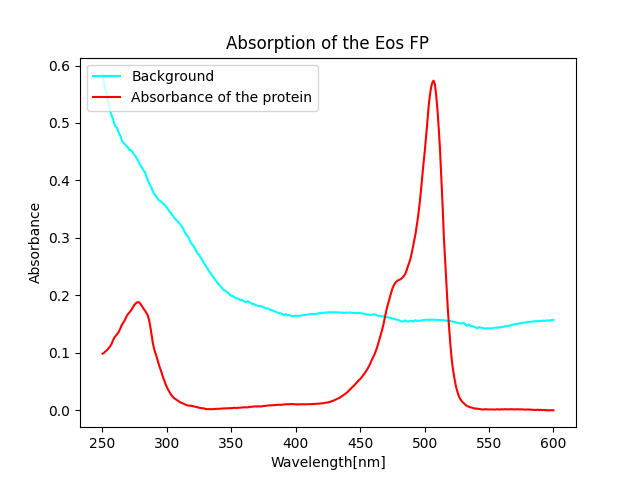
\includegraphics[width=\textwidth]{Figures/Absorption.png}
%    \caption{Absorption spectrum of purified Eos protein. The peaks at 280 nm and 506 nm correspond to.....}
%    \label{fig:absorption_spectrum}
%\end{figure}

\begin{figure}[htbp]
    \centering
    \begin{subfigure}[b]{0.45\textwidth}
        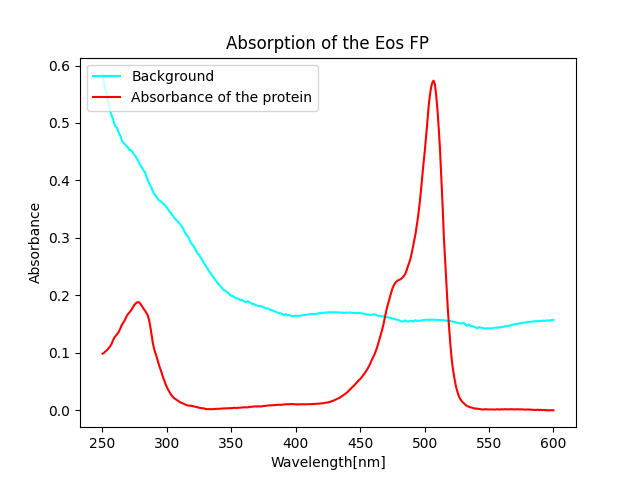
\includegraphics[width=\textwidth]{Figures/Absorption.png}
        \caption{Absorption spectrum (red) and the background (cyan)}
        \label{fig:sub1}
    \end{subfigure}
    \quad % Adjust spacing between subfigures as needed
    \begin{subfigure}[b]{0.45\textwidth}
        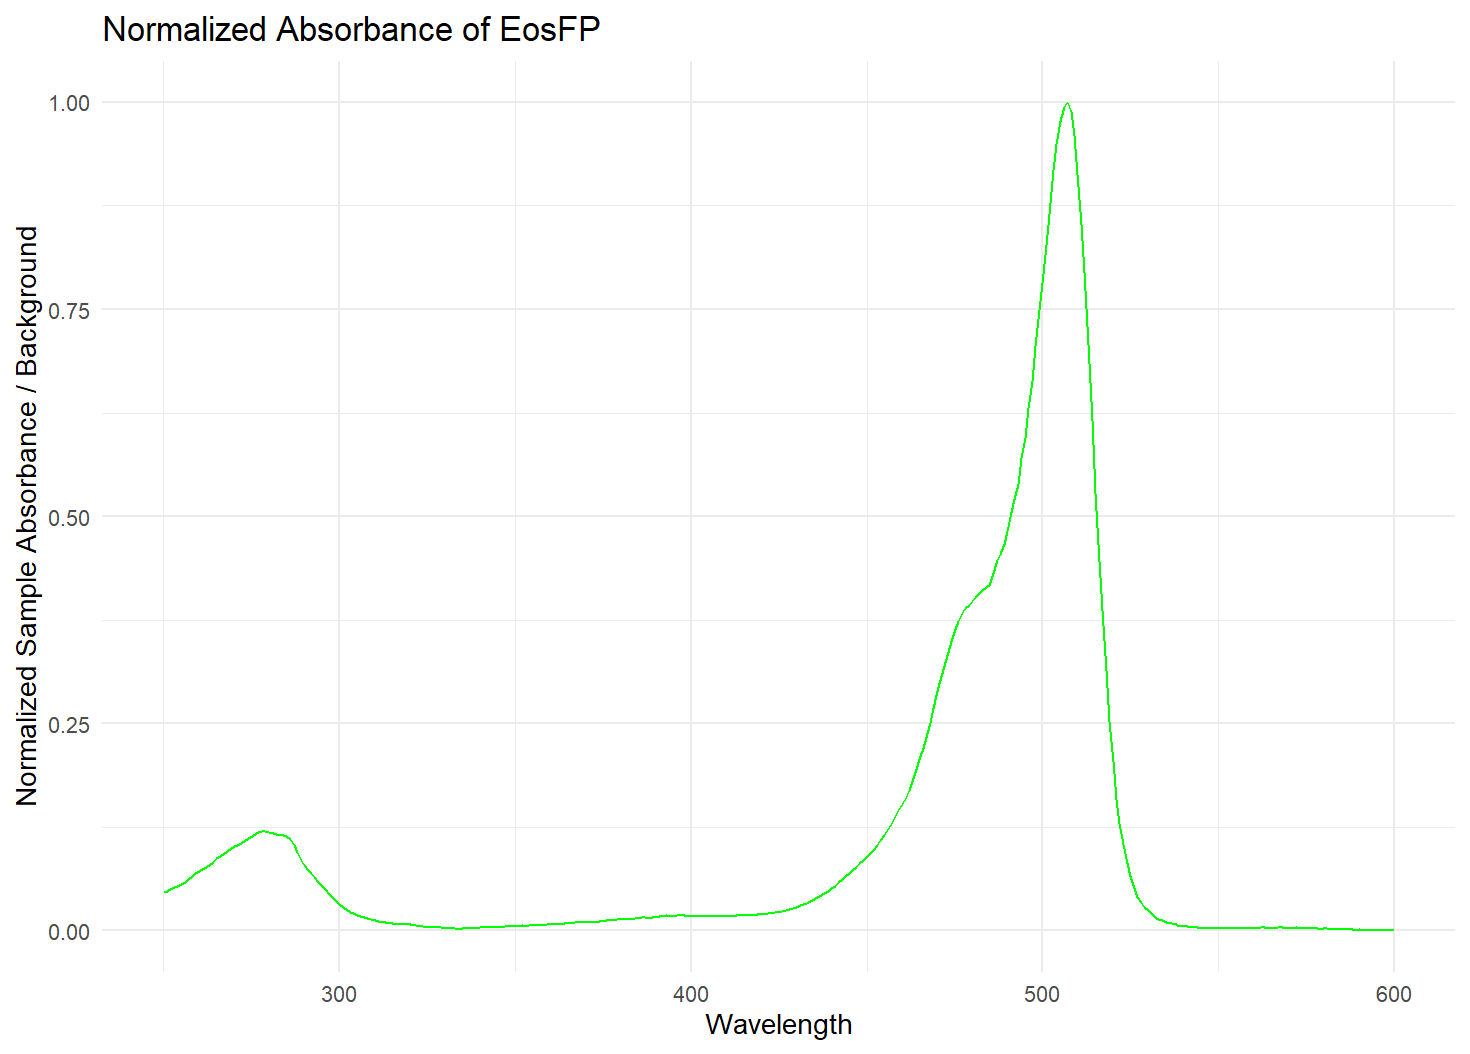
\includegraphics[width=\textwidth]{Figures/absorbance.png}
        \caption{Normalized and background-corrected absorption spectrum}
        \label{fig:sub2}
    \end{subfigure}
    \caption{The absorption spectrum of the purified Eos protein. }
    \label{fig:main}
\end{figure}
As is shown in Figure 3.1, the absorption spectrum of the Eos fluorescence protein has two significant absorption peaks around 280 nm and 510 nm. Referring to the published data\cite{D1CB00014D} and calculation, we acquired the extinction coefficient of the protein at 280 nm ($\epsilon_{280}$ = 27432.5 $\pm$ 62.5 $\mathrm{M^{-1}cm^{-1}}$) and 506 nm ($\epsilon_{506}$ = 72000 $\mathrm{M^{-1}cm^{-1}}$). The length of the cuvette is 1 cm. Thus, the concentration could be calculated using Beer-Lambert law.
\[
c_1 = \frac{A_{280}}{\epsilon_{280} \cdot d} = \frac{0.183}{27432 \times 1} = 6.67 \times 10^{-6} M
\]
\[
c_2 = \frac{A_{506}}{\epsilon_{506} \cdot d} = \frac{0.573}{72000 \times 1} = 7.96 \times 10^{-6} M
\]
The average concentration of the protein is $7.32 \times 10^{-6}$ M.\\
% Proof the changing rate of the green peak and the red peak are the same, by analyzing the movie of the photoconvertion experiment.
And the results of the photoconversion are shown in Figure 3.2 and 3.3. In Figure 3.2, we could clearly observed the intensity changes of the emission peaks from around 520 nm to around 580 nm (The time scale are displayed from blue to red). And we also plotted the change of wavelength over time at 516 nm (green) and 580 nm (red) to see the rate of the intensity change. The fitting result of two curves are as follows:
\[
I_{green} = 1.83 \times 10^{4} e^{-5.32\times 10^{-2} t}
\]
\[
I_{red} = 2.70 \times 10^{3} ln(t-7.81)
\]
And by calculating the rate of changing and plot (Figure 3.4), we could notice that the changing rate of the light intensity at 516 nm and 580 nm are close, which partially supported the theory of photoconversion.
\begin{figure}[h]
    \centering
    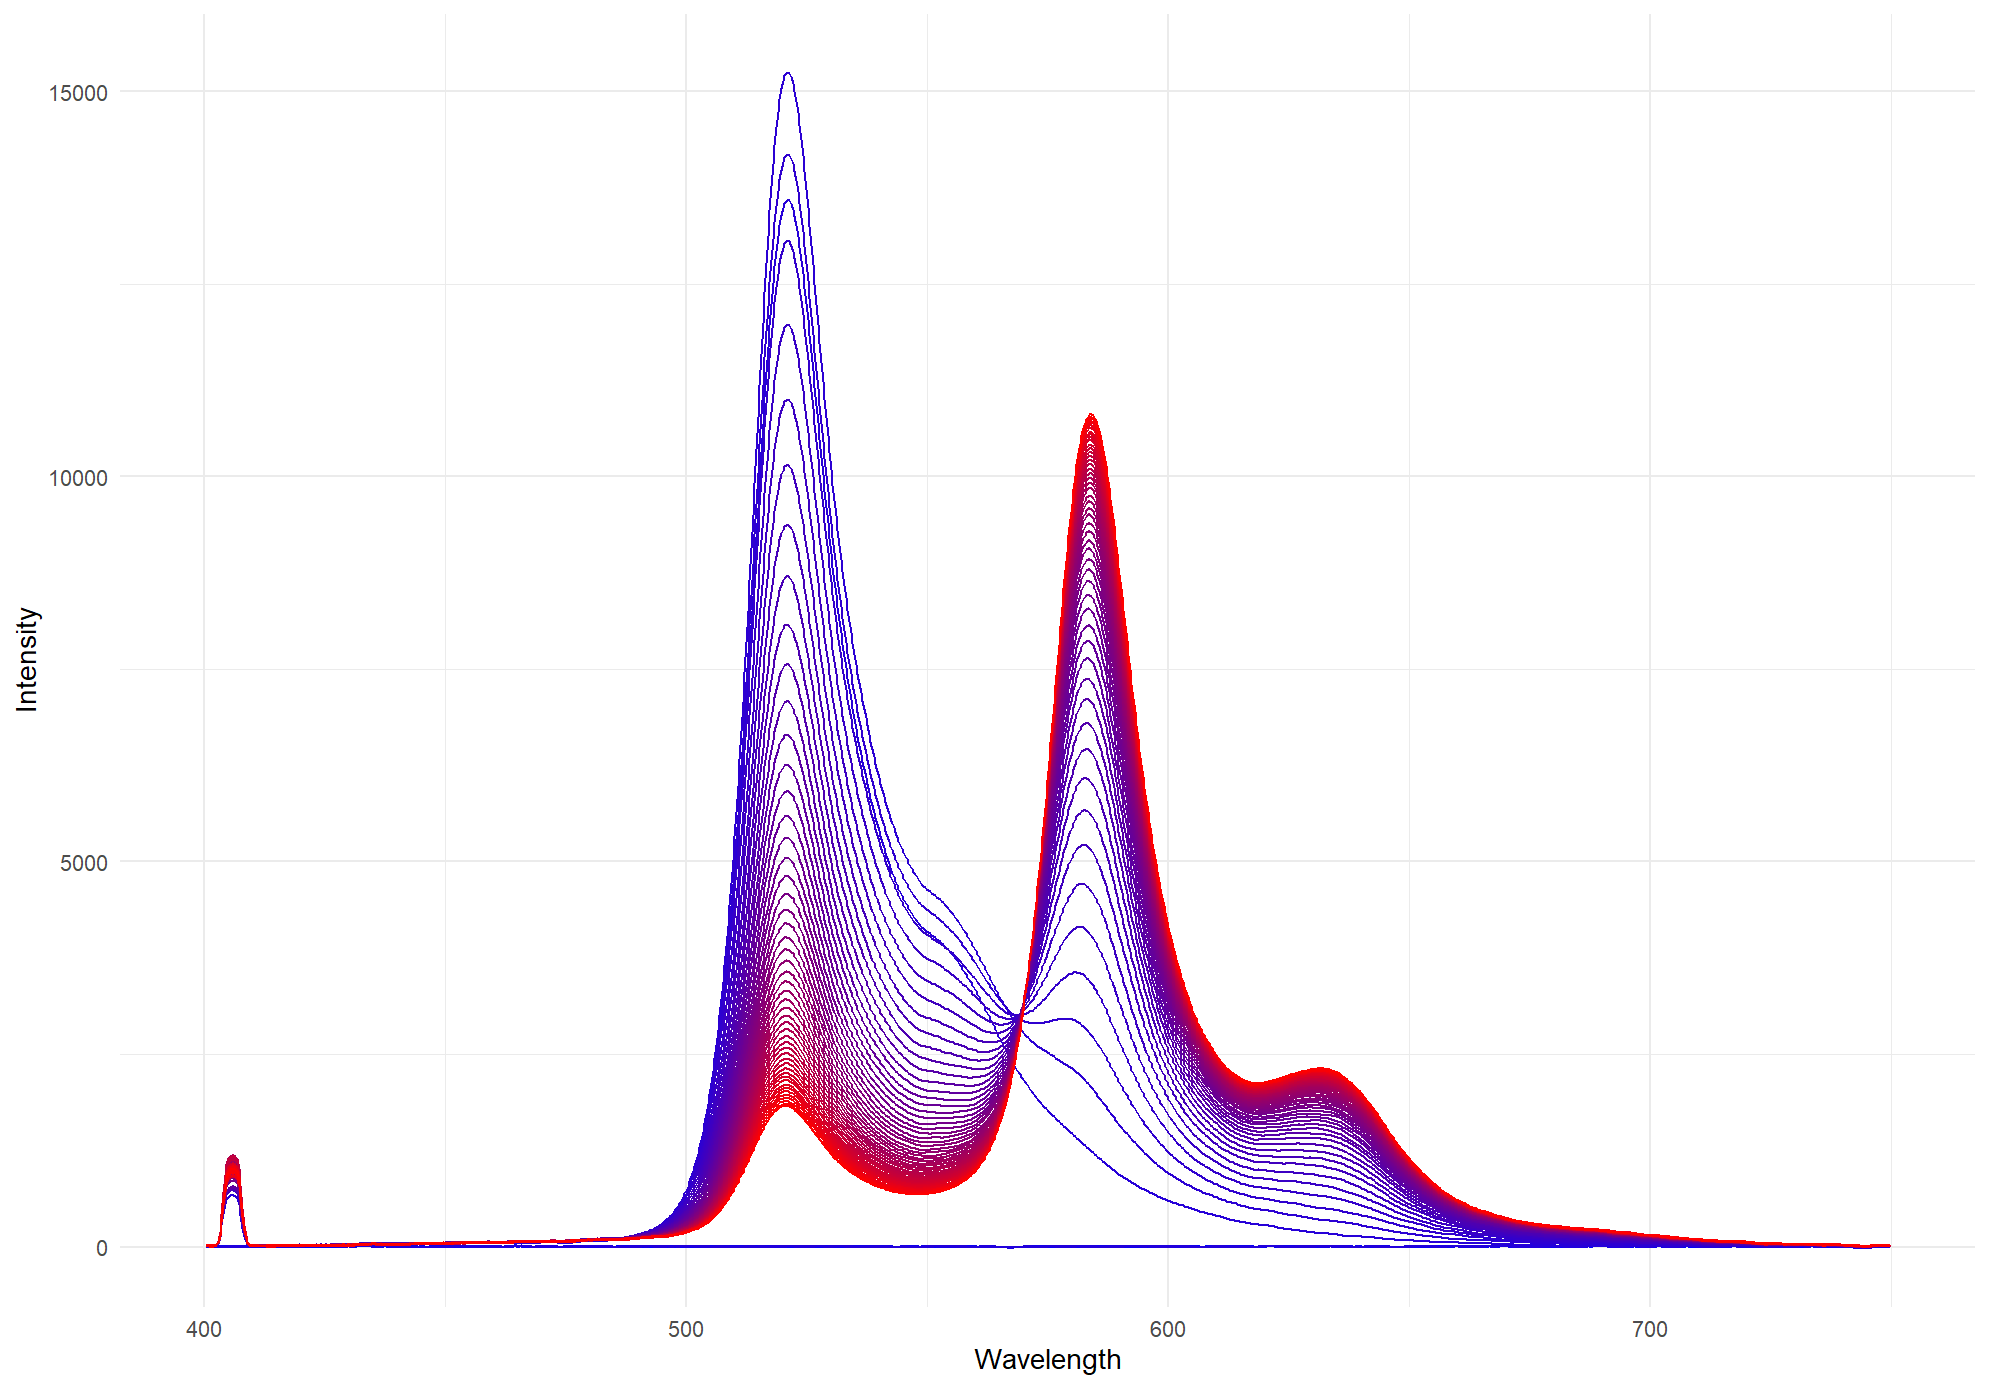
\includegraphics[width=0.9\textwidth]{Figures/conversion.png} 
    \caption{Photoconversion kinetics of Eos protein. The fluorescence intensities of the sample is plotted over time, from blue to red. Demonstrating on the left the small 405 nm peak produced by the excitation UV light, and the gradual decrease of the green peak at 516 and an increase of the red peak at 581 nm.}
    \label{fig:photoconversion}
\end{figure}

\begin{figure}[h]
    \centering
    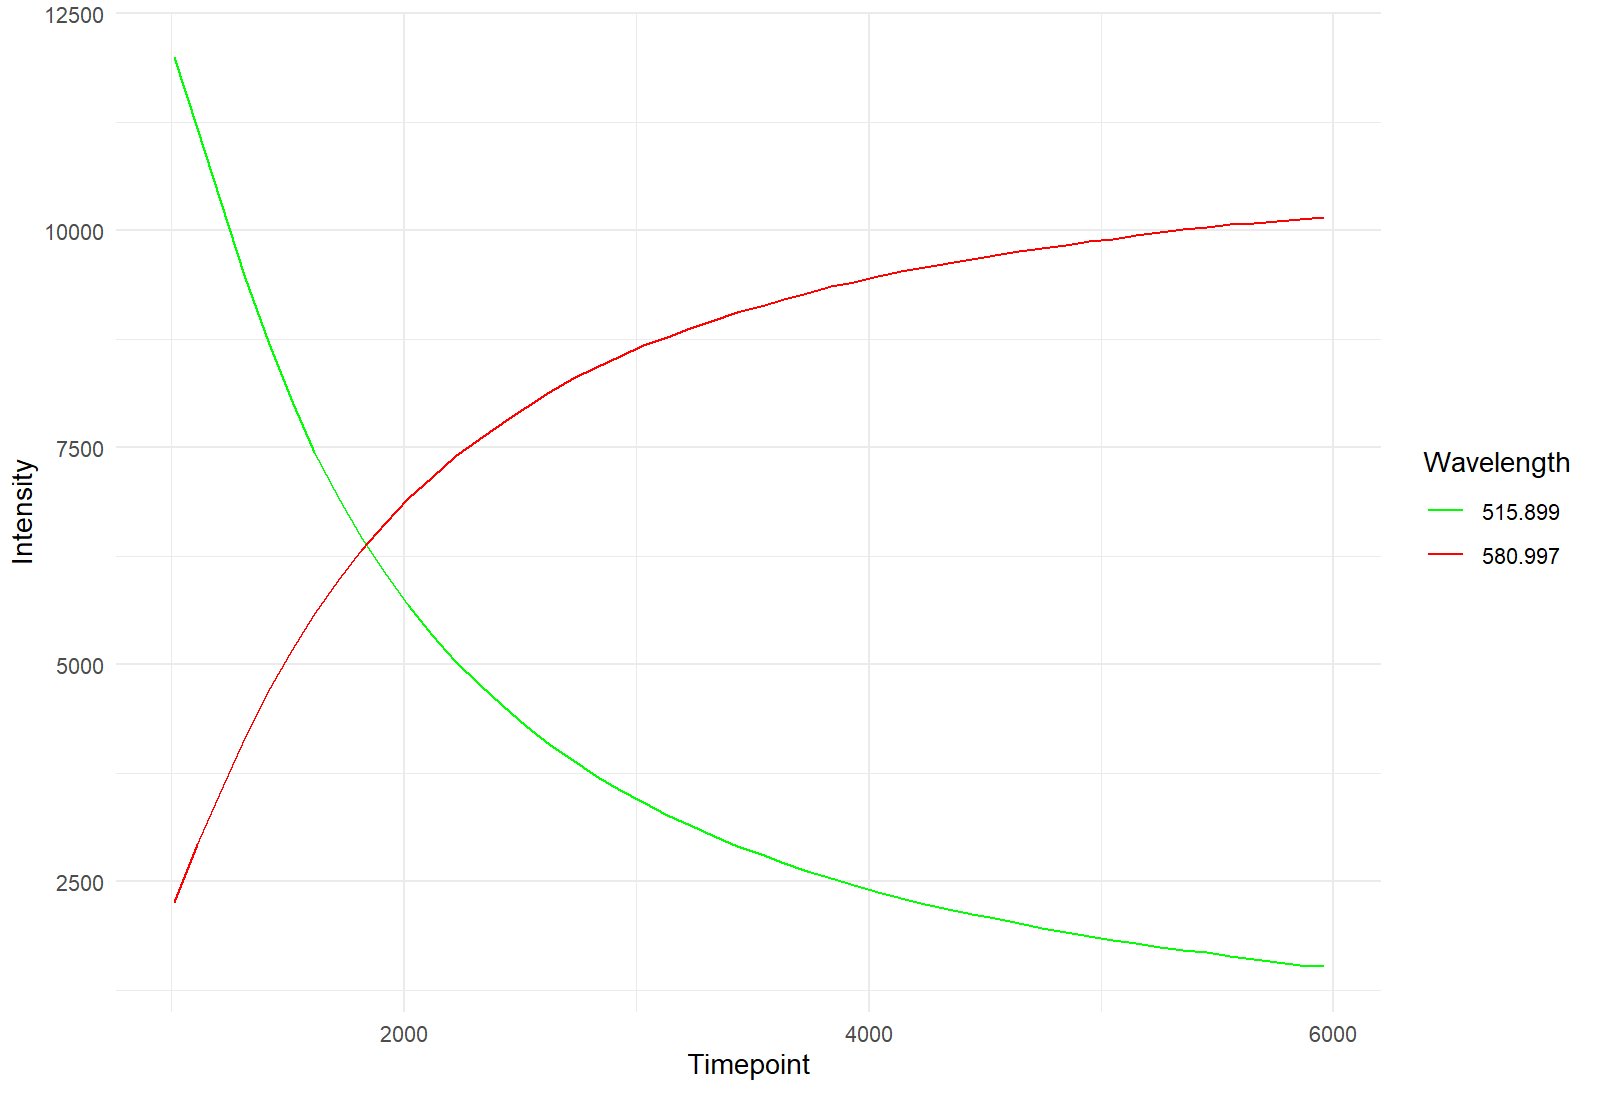
\includegraphics[width=0.9\textwidth]{Figures/Wavelengths intensity.png} 
    \caption{Emission Peaks as a function of Time showing that the the 516 nm peak decreases following an exponential decay and the 581 nm peak increases following a logarithmic function}
    \label{fig:photoconversion}
\end{figure}

\begin{figure}
    \centering
    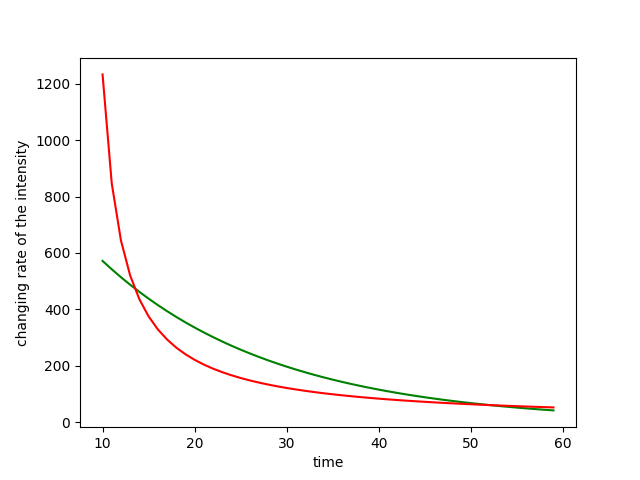
\includegraphics[width = 0.8\textwidth]{Figures/changing.png}
    \caption{The changing rate of the green light(fliped over) and the red light}
    \label{fig:enter-label}
\end{figure}
\chapter{Discussion}
\label{cha:Discussion}

% Opposing values for the 280nm between computed and experimental, we chose the computed value since the literature provided only circumstantial evidence and no reference or result for the claim
In the calculation of the protein concentration, we need the extinction coefficient of Eos FP at 280 nm and 506 nm. On the one hand, published data of the extinction coefficient at 506 nm could be easily acquired\cite{doi:10.1073/pnas.0403668101}. On the other hand, searching for the extinction coefficient of Eos FP at 280 nm was difficult, since the literature provided only circumstantial evidence and no reference or result for the claim. Instead of acquiring the extinction coefficient directly from the experiment, we could also compute the extinction coefficient by the protein structure and its sequence information, since we know the effects of different amino acids and their bonds on the extinction coefficient. According to the published article\cite{extinction_coefficient}, this calculation provides a good result, we decided to use the calculated extinction coefficient of Eos FP at 280 nm instead of the published value.\\


%UV light changed the molecule structure of the EosFP, the new pi bond changes the fluorescence area and makes the green-to-red shift possible. Explain it with the box theory.
\begin{figure}[H]
    \centering
    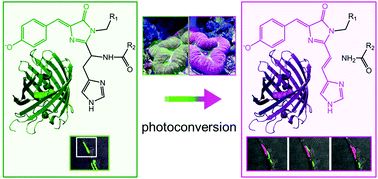
\includegraphics[width = 0.8\textwidth]{Figures/bond_change.png}
    \caption{The chemical structure change of Eos FP being exposed to UV light\cite{D1CB00014D}}
    \label{fig:enter-label}
\end{figure}

The mechanics of the photoconversion can be explained with reference to Figure 4.1. As shown in the figure, before the protein is exposed to UV light, the major fluorescent group of the protein (connected by conjugated pi bonds) is labeled in green. When the UV light interacts with the protein, the amide group acquires electrons and releases them from the protein, which reduces the carbon atom and extends the area connected by conjugated pi bonds. This extension increases the emission region of the protein, thereby changing the wavelength of the emitted light. The shift from green to red can be explained by the particle-in-a-box theory (Figure 4.2). According to this theory, the energy of the emitted photons is determined by the energy level and the length of the box. In our case, the length of the box is proportional to the length of the area connected by conjugated pi bonds. Based on the energy formula in Figure 4.2, assuming that all the emissions happen between the same energy levels, the longer the length, the lower the energy, and since energy is inversely proportional to the wavelength (E $\propto$ 1/$\lambda$), a longer length results in an increased wavelength. Calculations show that this redshift places the wavelength in the red light region, which aligns well with our experimental results.
\begin{figure}[H]
    \centering
    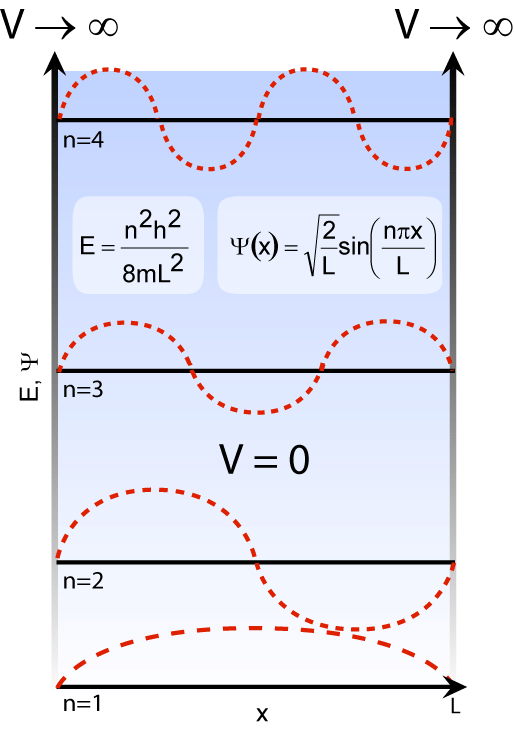
\includegraphics[width = 0.8\textwidth]{Figures/box_theory.png}
    \caption{The sketch of the energy level in the particle-in-box theory\cite{box}}
    \label{fig:enter-label}
\end{figure}
%show the image where you can see the orange stripe in the green liquid just to make it more evident as a point
\begin{figure}[H]
    \centering
    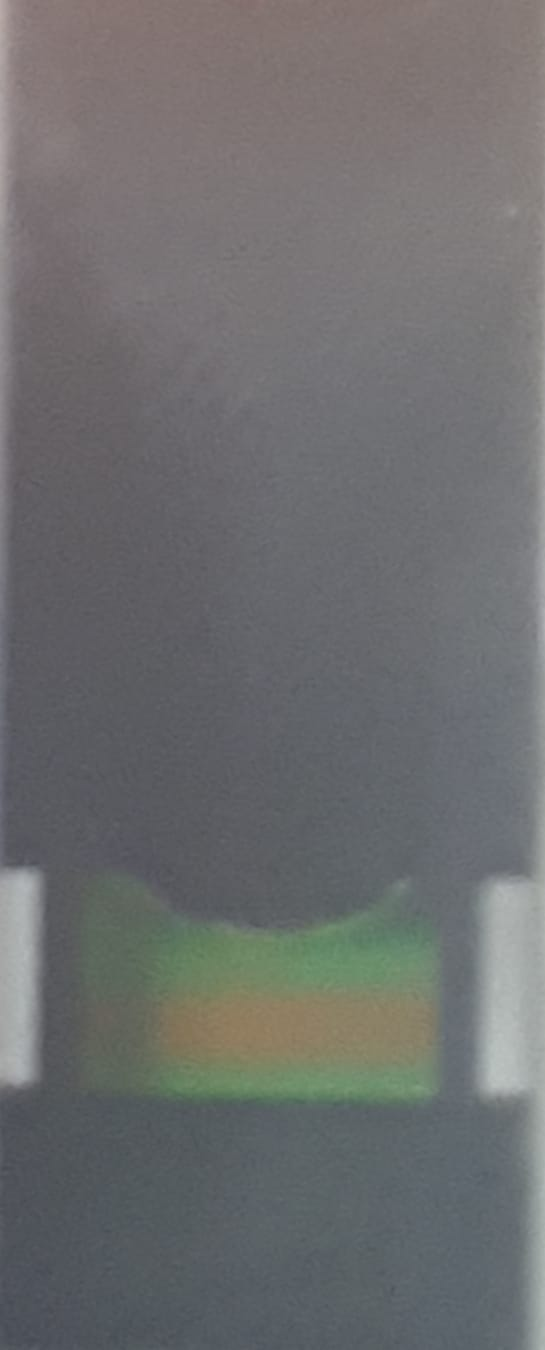
\includegraphics[width = 0.15\textwidth]{Figures/WhatsApp Image 2024-06-24 at 10.49.14.jpeg}
    \caption{The cuvette showing a clear distinction between the solution exposed to UV and the the one not exposed, providing visual proof of the photoconversion}
    \label{fig:enter-label}
\end{figure}

\printbibliography
\end{document}